\section{Denoising Diffusion Probabilistic Models}

Diffusion models generate samples by starting from random noise and iteratively denoising it, guided by a learned model. Two common sampling approaches are:

\begin{enumerate}
    \item \textbf{DDPM (Denoising Diffusion Probabilistic Models):} A step-by-step Markovian reverse process that typically uses many steps but ensures high-quality reconstructions.
    \item \textbf{DDIM (Denoising Diffusion Implicit Models):} A non-Markovian approach allowing deterministic sampling and fewer steps, making sampling faster.
\end{enumerate}

\subsection*{Background}

Consider a forward diffusion process that gradually adds Gaussian noise to an initial image $x_0$ over $T$ steps. Define a noise schedule $\{\beta_t\}$ and set $\alpha_t = 1 - \beta_t$.

\subsubsection*{Forward Process}
The forward process is:
\[
    q(x_t \mid x_{t-1}) = \calN(x_t; \sqrt{\alpha_t}x_{t-1}, (1-\alpha_t)I).
\]

After many steps, $x_T$ is approximately isotropic Gaussian noise.

\subsubsection*{Reverse Process}
We seek to reverse the forward process:
\[
    p_\theta(x_{t-1} \mid x_t) = \calN(x_{t-1}; \mu_\theta(x_t, t), \sigma_t^2 I).
\]

The model (e.g., a \href{https://arxiv.org/pdf/1505.04597}{UNet}) predicts the noise $\epsilon_\theta(x_t, t)$, from which we can estimate the original sample:
\[
x_0 \approx \frac{x_t - \sqrt{1-\bar{\alpha}_t}\,\epsilon_\theta(x_t,t)}{\sqrt{\bar{\alpha}_t}},
\]
where $\bar{\alpha}_t = \prod_{s=1}^t \alpha_s$.

\begin{enumerate}[label=(\alph*)]
    \item \points{4a} \textbf{Sampling using Vanilla DDPM and DDIM}

For \href{https://arxiv.org/pdf/2006.11239}{DDPM}, the posterior distribution of $x_{t-1}$ given $x_t$ and $x_0$ is known:
\[
    q(x_{t-1} \mid x_t, x_0) = \calN(x_{t-1}; \tilde{\mu}_t, \tilde{\beta}_t I),
\]
with
\[
    \tilde{\mu}_t = \frac{\sqrt{\bar{\alpha}_{t-1}}\beta_t}{1-\bar{\alpha}_t} x_0 
    + \frac{\sqrt{\alpha_t}(1-\bar{\alpha}_{t-1})}{1-\bar{\alpha}_t} x_t,
\]
and
\[
    \tilde{\beta}_t = \frac{1-\bar{\alpha}_{t-1}}{1-\bar{\alpha}_t}\beta_t.
\]

By iterating these steps backward from $T$ to $0$ and adding Gaussian noise at each step (except $t=0$), we reconstruct a clean sample from pure noise.

Given the provided code in the \texttt{sample.py} file, please implement the following functions:

\begin{itemize}
    \item \texttt{get\_timesteps}
    \item \texttt{predict\_x0}
    \item \texttt{compute\_forward\_posterior\_mean}
    \item \texttt{compute\_forward\_posterior\_variance}
\end{itemize}

To generate mnist sample run: 
\begin{lstlisting}[language=bash]
    python run_sampling.py --dataset mnist --experiment ddpm
\end{lstlisting}

Run the experiment to generate few samples with \textbf{num\_steps}=5, 10, 20, 50 and provide a comment. 
\textbf{Hint: }Once we stabilize the quality at 10, we notice that the result is always almost the same.

If you have enough time and resources you can run to generate 256x256 faces samples

\begin{lstlisting}[language=bash]
    python run_sampling.py --dataset faces --experiment ddpm
\end{lstlisting}

You will generate samples thast look like:

\begin{figure}[h]
    \centering
    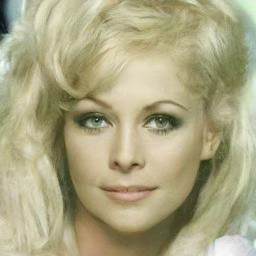
\includegraphics[width=0.5\textwidth]{./figures/ddpm_steps1000_seed42_img_0}
    \caption{DDPM samples for Celebrity dataset}
\end{figure}

\textbf{DDIM Sampling}

DDIM sampling provides a shortcut:
\[
x_{t-1} = \sqrt{\bar{\alpha}_{t-1}}x_0 + \sqrt{1-\bar{\alpha}_{t-1}}\epsilon_\theta(x_t,t).
\]
This is a special case of the general formula (16) in \href{https://arxiv.org/pdf/2010.02502}{the DDIM paper} where $\eta = 0$.

Run the \texttt{ddim\_inference} to implement the DDIM update following the previous equation.

To generate mnist sample run: 
\begin{lstlisting}[language=bash]
    python run_sampling.py --dataset mnist --experiment ddim
\end{lstlisting}

Run the experiment to generate few samples with \textbf{num\_steps}=5, 10, 20, 50 and provide a comment. 
\textbf{Hint: }Once we stabilize the quality at 10, we notice that the result is always almost the same.

If you have enough time and resources you can run to generate 256x256 faces samples

\begin{lstlisting}[language=bash]
    python run_sampling.py --dataset faces --experiment ddim
\end{lstlisting}

You will now generate samples thast look like:

\begin{figure}[H]
    \centering
    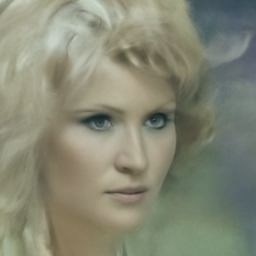
\includegraphics[width=0.5\textwidth]{./figures/ddim_steps10_seed42_img_0}
    \caption{DDIM samples for Celebrity dataset}
\end{figure}

    \item \points{4b} \textbf{DDIM as Markovian Process}

We wish to introduce a Markovian variant of DDIM, we can incorporate a noise term at each step to make it probabilistic. 
Consider a parameter $\sigma_t$ that controls the amount of noise injected back into the process. By doing so, we can smoothly transition 
from a DDIM-like deterministic sampler (when $\sigma_t=0$) to a full stochastic, Markovian process (when $\sigma_t>0$).


To make the previous step Markovian, we introduce a noise term with variance controlled by $\sigma_t$, which is described by the formula (16) 
in \href{https://arxiv.org/pdf/2010.02502}{the DDIM paper}. Let $z \sim \mathcal{N}(0,I)$ be a standard Gaussian noise sample. 
The Markovian variant of the DDIM update can be written as:

\[
x_{t-1} =
\sqrt{\bar{\alpha}_{t-1}} x_0
+ 
\underbrace{\sqrt{1 - \bar{\alpha}_{t-1} - \sigma_t^2}\,\epsilon}_{\text{\texttt{predict\_sample\_direction}}} 
+ 
\underbrace{\sigma_t z}_{\text{\texttt{stochasticity\_term}}}.
\]

Please implement the following functions from the :
\begin{itemize}
    \item \texttt{get\_stochasticity\_std}
    \item \texttt{predict\_sample\_direction}
    \item \texttt{stochasticity\_term}
\end{itemize}

to accurately reproduce the update method described in the \href{https://arxiv.org/pdf/2010.02502}{the DDIM paper} by the formulas (12) and (16).

Run the experiment to generate few samples with \textbf{eta}=0, 0.2, 0.5, 0.75, 1 for \textbf{num\_steps} = 10 and provide a comment.

    \item \input{04-ddpm-ddim/03-compare}
\end{enumerate}